\documentclass{resume}

\usepackage[left=0.75in,top=0.6in,right=0.75in,bottom=0.6in]{geometry}


\name{Nguyen Ba Vuong}


% \def\nameskip{\bigskip}
% \def\sectionskip{\medskip}

\begin{document}

  %%% Overview
  %%% ------------------------------------------------------------

  \noindent\begin{minipage}{0.8\textwidth}% adapt widths of minipages to your needs
    I'm an experienced developer interested in building usable, useful, well-constructed websites and applications. 
    Knowledgeable of all the development cycle stages, have a good command of coding languages and excellent problem-solving skills.
    Interested in continuation of learning and cooperation with excellent people.
    Experience working on Full-stack Javascript Applications, using some of the latest technologies, including:
    ReactJs| React Native| NodeJs| JestJs and more.
    \end{minipage}%
    \hfill%
    \begin{minipage}{0.1\textwidth}\raggedright
      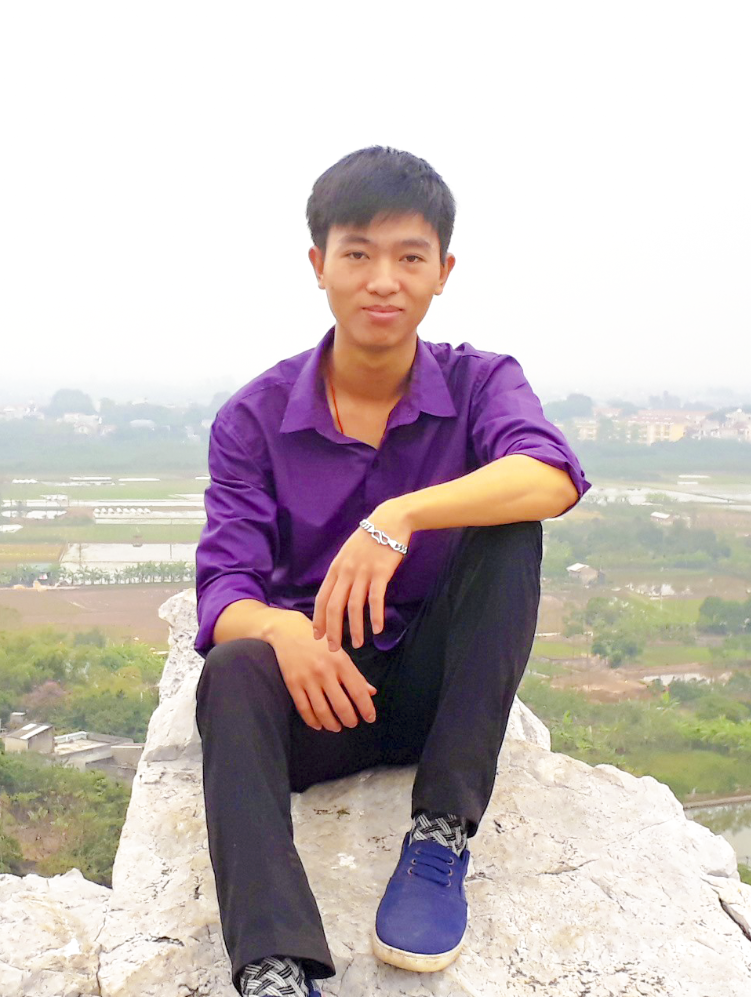
\includegraphics[width=3cm, height=4cm]{profile}
    \end{minipage}

  %%% Skills
  %%% ------------------------------------------------------------
  \begin{rSection}{Technical skill}
    \begin{rSubsection}{}{}{}{}
      \item Strong JavaScript experience, both OO and functional patterns.
      \item Solid experience with TypeScript.
      \item Expert knowledge of ReactJs, NextJs, React Native
      \item Experience with common React UI library: MaterialUI, React Bootstrap, Native Base.
      \item Experience with common React state management: Context, Redux, Mobx
      \item Have experience with build native module for React Native.

      \item API development and design with Node.js: Koa, Express, NestJs
      \item Experience with GraphQL, Rest Full Api
      \item Experience with both NoSQL databases (MongoDB) and SQL databases (PostgreSQL).

      \item Have experience with Git to manage source control.
      \item Comfortable with CLI and related software (vim, zsh).
      \item Understanding of SDLC and Software Architecture.
      \item Good knowledge of OOP, OOA, Design Pattern and SOLID principles
      \item Familiarity with mobile application build/roll out process, and native build tool.
    \end{rSubsection}
  \end{rSection}
  
  %%% Exp
  %%% ------------------------------------------------------------
  \begin{rSection}{Experience}
    \begin{rSubsection}{MTT Software Company}{August 2017 - Present}{Fullstack JavaScript Developer}{}
      \item Develop dynamic and responsive website, mobile applications with clean interface and simple.
      \item Develop project concepts and maintain optimal workflow.
      \item Participate in database design and api backend tasks.
      \item Carry out quality assurance unit tests to discover errors and optimize usability.
      \item Optimized website/application usability.
      \item Completed programming and development tasks of different difficulty levels.
    \end{rSubsection}
     
    \begin{rSubsection}{}{}{My accomplished projects at MTT}{}
      \item \href{https://mttjsc.com/}{\emph{\bfseries{MTT Website}}}: An affiliate website for MTT.
      \item \emph{\bfseries{Nailshop Ecosystem}} (\href{https://play.google.com/store/apps/developer?id=MTT+Software+Company+LTD}{\emph{Android}}/\href{https://apps.apple.com/us/developer/mttjsc/id1250334932}{\emph{IOS}}): 
      An ecosystem to provide service for nailshop owner manager their staff, schedule their working timeline, get monthly statistic report and connect customer with shops.
      \item \href{https://app.scnt.me/}{\emph{\bfseries{Scentronix}}}: A PWA web app which help people select their favorite perfume ingredients to make their own one.
      \item {\emph{\bfseries{Lifeguard}}}: An IOS application which used to scan workers' protective equipments before they start their jobs. 
      \item {\emph{\bfseries{PAA Attendance}}}: System which used to auto attendance with camera at university
      \item {\emph{\bfseries{Shuttle Bus}}}: Mobile application which used to attendance pupils in school bus
      \item \href{https://dev.console.phenikaa.cloud/}{\emph{\bfseries{Cloud Platform Computer Vision}}}: An web application provide api for recognition: face detect, face compare, face search, face id, video analysis, voices,...
    \end{rSubsection}
  \end{rSection}



  {}{}
  %%% Others
  %%% ------------------------------------------------------------
  \begin{rSection}{Education}
    {\bf Hanoi University of Industry} (2015-2019) \\ 
    { Specialized: Computer Science } \\
  \end{rSection}

  %%% Personal details
  %%% ------------------------------------------------------------
  \begin{rSection}{Contacts}
    \PersonalEntry{\faSkype}{\url{https://join.skype.com/invite/ko61wsOQvB9S}}
    \PersonalEntry{\faLinkedin}{\url{https://www.linkedin.com/in/vuong-nguyen-ba-051b9b1a3/}}
    \PersonalEntry{\faGithub}{\url{https://github.com/bavuongvng}}
    \PersonalEntry{\faGlobe}{\url{https://vuonghnit.github.io}}
    \PersonalEntry{\faAt}{\href{mailto:bavuongvng@gmail.com}{bavuongvng@gmail.com}}
    \PersonalEntry{\faPhone}{(+84) 39 706 2438}
    \PersonalEntry{\faBirthdayCake}{1997}
    \PersonalEntry{\faMapMarker}{Hanoi}
  \end{rSection}

\end{document}
